\documentclass[10pt,aspectratio=43,mathserif,table]{beamer} 
%  设置为 Beamer 文档类型,设置字体为 10pt,长宽比为16:9,数学字体为 serif 风格
\batchmode
\usepackage{graphicx}
\usepackage{subfigure}
\usepackage{fontspec}

\setmainfont{Harding Text Web Regular Regular.ttf}
\usepackage{diagbox} % 表头斜线分区
\usepackage{unicode-math}
\usefonttheme{serif}
% \setmathrm{Harding Text Web Regular Regular.ttf} % 设置数学字体为 Times New Roman
% \setmathfont{TeX Gyre Termes Math} % 如果您使用 XeLaTeX 或 LuaLaTeX 编译,可以使用其他数学字体
% \setmathtt{Courier New} % 设置等宽字体为 Courier New
% \setboldmathrm{Times New Roman}
% \setmathfont{TeX Gyre Termes Math}[version=bold] % 设置粗体数学字体
% \setmathfont{TeX Gyre Termes Math}[range={\mathit}]


\usetheme{Berlin} %主题
\setbeamertemplate{page number in head/foot}[pagenumber]
%\usecolortheme{sustech} %主题颜色

\usepackage[ruled,linesnumbered]{algorithm2e}

\usepackage{fancybox}
\usepackage{xcolor}
\usepackage{listings}
\usepackage{multicol}
\usepackage{booktabs}
\usepackage{colortbl}

\newcommand{\Console}{Console}
\lstset{ %
	backgroundcolor=\color{white},   % choose the background color
	basicstyle=\footnotesize\rmfamily,     % size of fonts used for the code
	columns=fullflexible,
	breaklines=true,                 % automatic line breaking only at whitespace
	captionpos=b,                    % sets the caption-position to bottom
	tabsize=4,
	commentstyle=\color{mygreen},    % comment style
	escapeinside={\%*}{*)},          % if you want to add LaTeX within your code
	keywordstyle=\color{blue},       % keyword style
	stringstyle=\color{mymauve}\ttfamily,     % string literal style
	numbers=left, 
	%	frame=single,
	rulesepcolor=\color{red!20!green!20!blue!20},
	% identifierstyle=\color{red},
	language=c
}


\definecolor{mygreen}{rgb}{0,0.6,0}
\definecolor{mymauve}{rgb}{0.58,0,0.82}
\definecolor{mygray}{gray}{.9}
\definecolor{mypink}{rgb}{.99,.91,.95}
\definecolor{mycyan}{cmyk}{.3,0,0,0}

%题目,作者,学校,日期
\title{Paper Reading}
%\subtitle{\fontsize{9pt}{14pt}\textbf{跨临界分岔}}
\author{Speaker: Yichen Lu\quad \newline  \newline \quad }
\institute{\fontsize{8pt}{14pt}}
\date{\today}
\newcommand{\concept}{Paper Reading}

%学校Logo
%\pgfdeclareimage[height=0.5cm]{sustech-logo}{sustech-logo.pdf}
%\logo{\pgfuseimage{sustech-logo}\hspace*{0.3cm}}

\AtBeginSection[]
{
	\begin{frame}<beamer>
	\frametitle{\textbf{Contents}}
	\tableofcontents[currentsection]
\end{frame}
}
% \beamerdefaultoverlayspecification{<+->}
% -----------------------------------------------------------------------------
\begin{document}
% -----------------------------------------------------------------------------
% \frame{\titlepage}

\section{Chiral Active Matter}

\begin{frame}
    \centering
    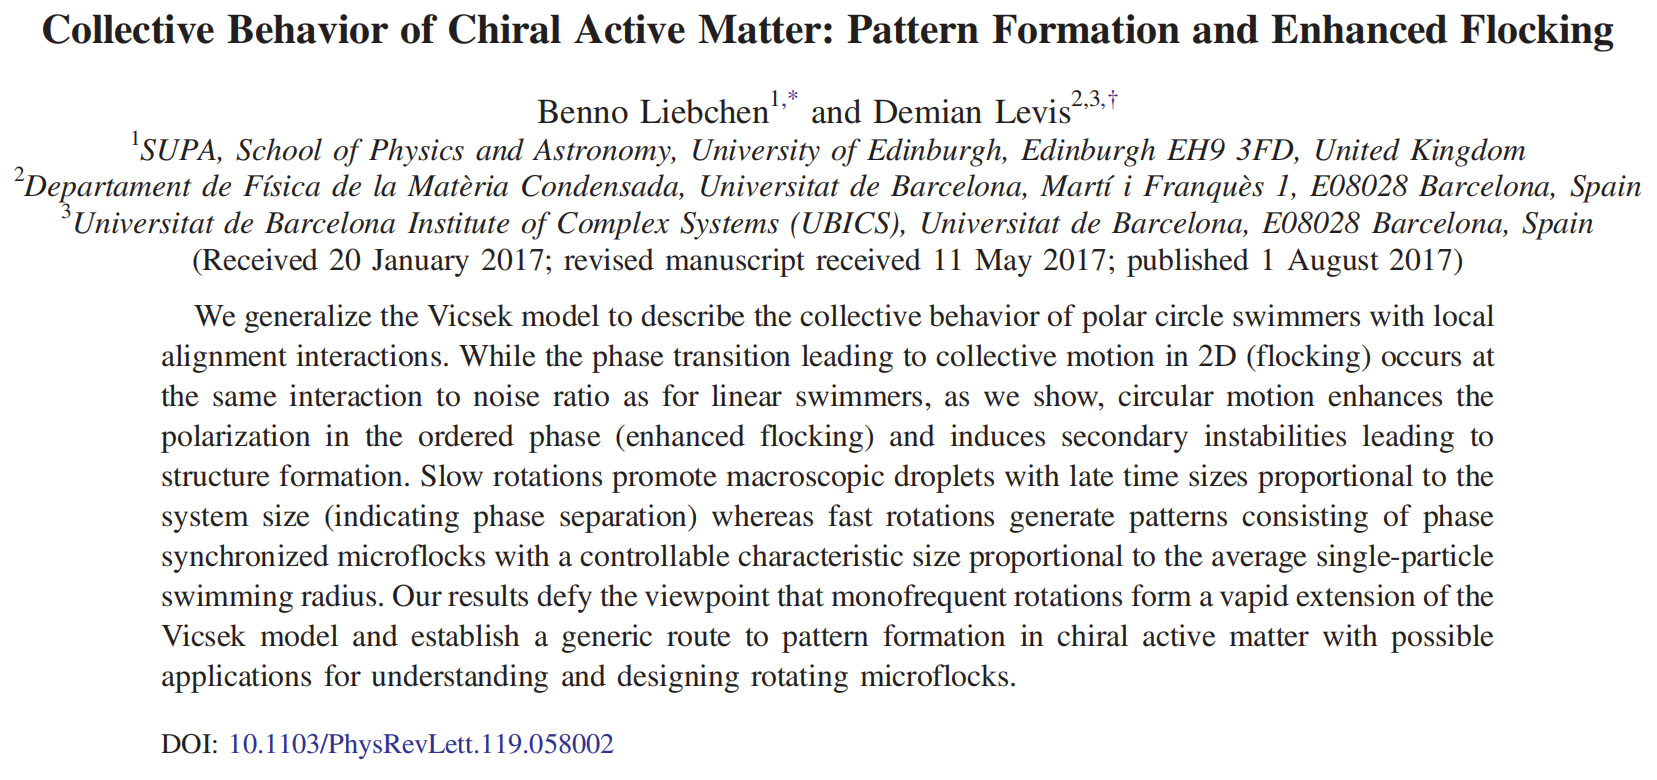
\includegraphics[width=\textwidth]{figs/title1.png}
\end{frame}

\begin{frame}
    \begin{multicols}{2}
        {
        \small
        $$
        \begin{aligned}
            \dot{\mathbf{r}}_i&=v\left[ \begin{array}{c}
            \cos \theta _i\\
            \sin \theta _i\\
        \end{array} \right]\\
            \dot{\theta}&=\omega +\frac{K}{\pi R_{\theta}^{2}}\sum_{j\in \partial _i}{\sin \left( \theta _j-\theta _i \right) +\sqrt{2D_r}\eta _{\boldsymbol{i}}}\\
        \end{aligned}
        $$
        $\eta_i(t)$ is a unit-variance Gaussian white noise with zero mean.
        
        $$ $$
        
        {
            \small
            To reduce the parameter space to model's essential dimensions, the authors choose space and time units as $R_{\theta}$ and $D_r^{-1}$. 
            Four dimensionless control parameters:
        }
        \begin{itemize}
            \item $\rho _0=NR_{\theta}^{2}/L^2$, the particle density
            \item $\mathrm{Re}_r=v/\left( D_rR_{\theta} \right) $, the P\'{e}clet number, measuring the persistence length in units of the alignment interaction range
            \item $g=K/\left( \pi R_{\theta}^{2}D_r \right) $, the alignment strength
            \item $\Omega=\omega/D_r$, comparing alignment and rotational frequencies with the rotational diffusion rate
        \end{itemize}

        }
    \end{multicols}
\end{frame}

\begin{frame}
    \centering
    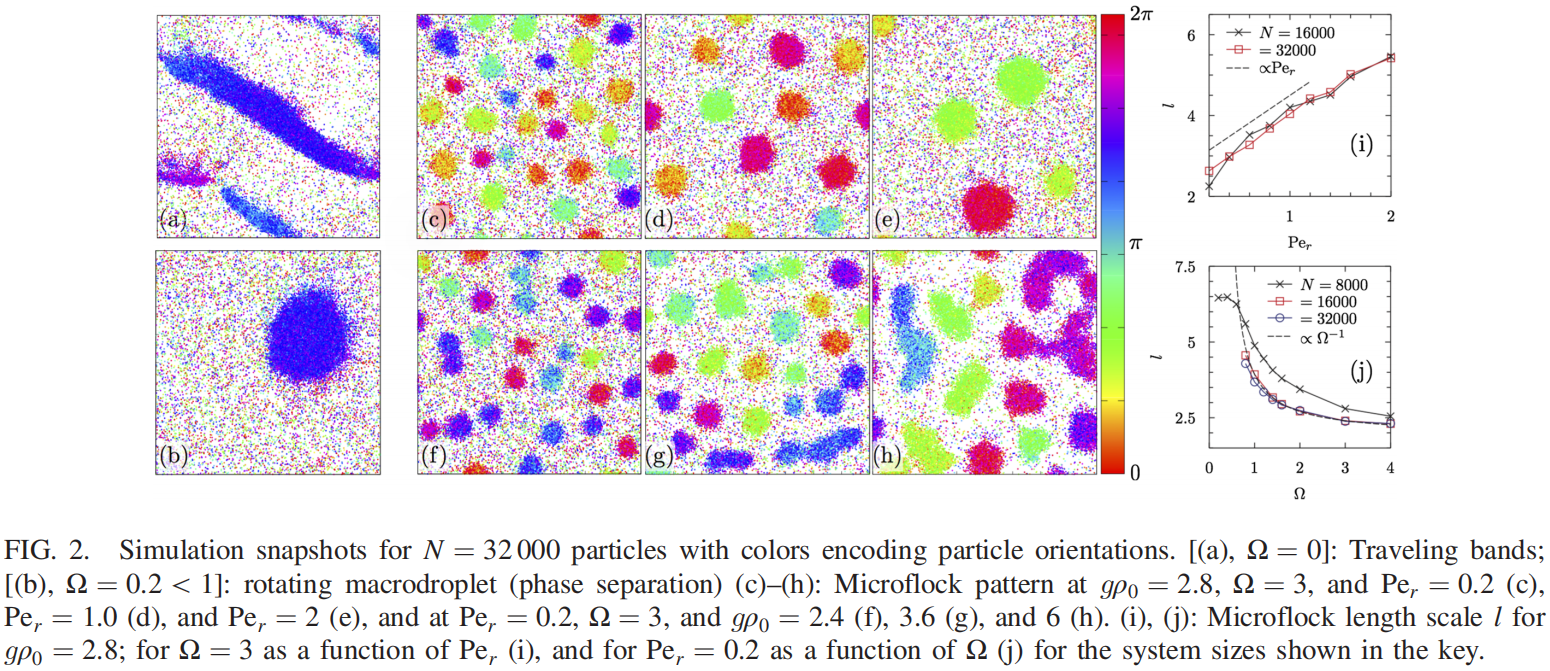
\includegraphics[width=0.95\textwidth]{figs/p1_f2.png}
    \begin{multicols}{2}
        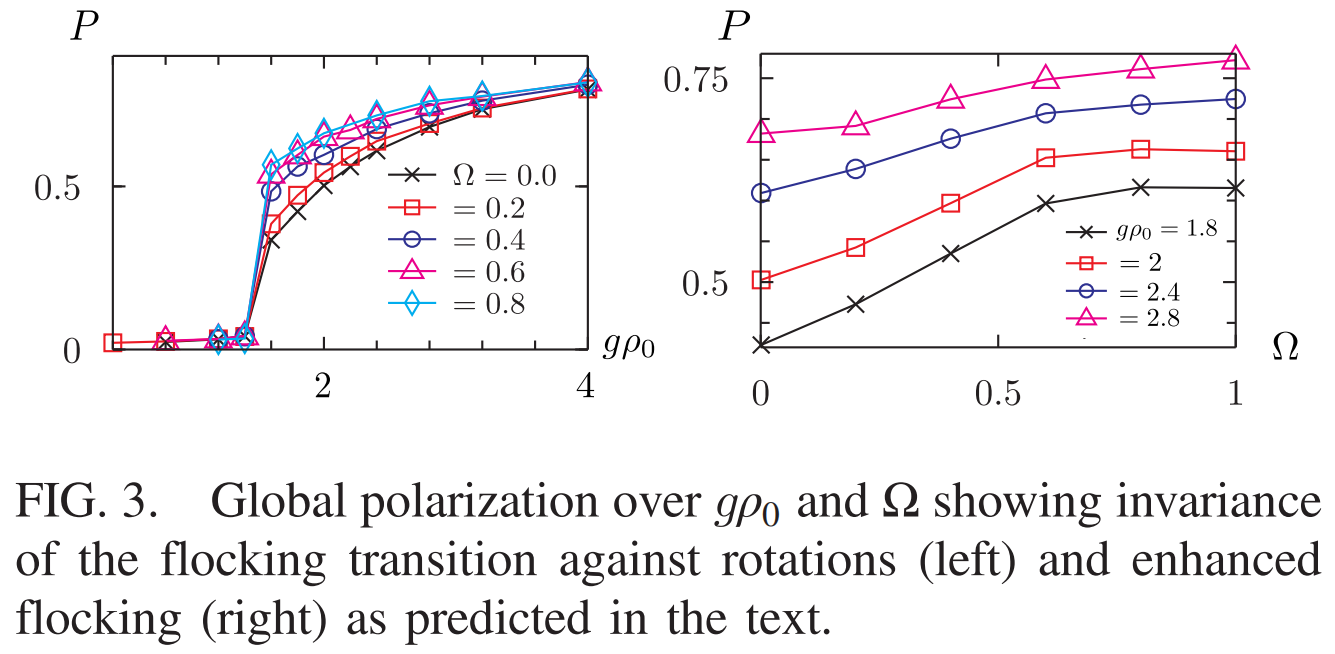
\includegraphics[width=0.5\textwidth]{figs/p1_f3.png}

        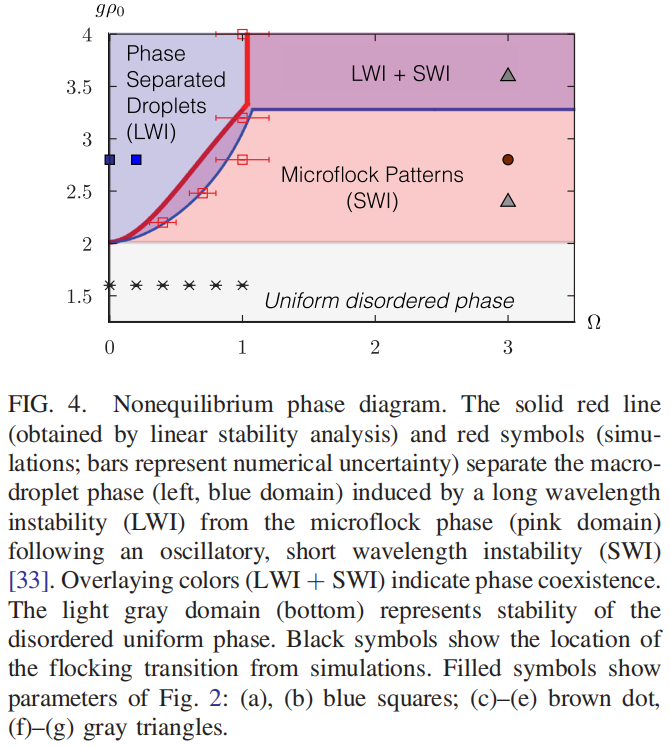
\includegraphics[width=0.5\textwidth]{figs/p1_f4.png}
    \end{multicols}
\end{frame}

\section{Pulsating Active Matter}

\begin{frame}
    \centering
    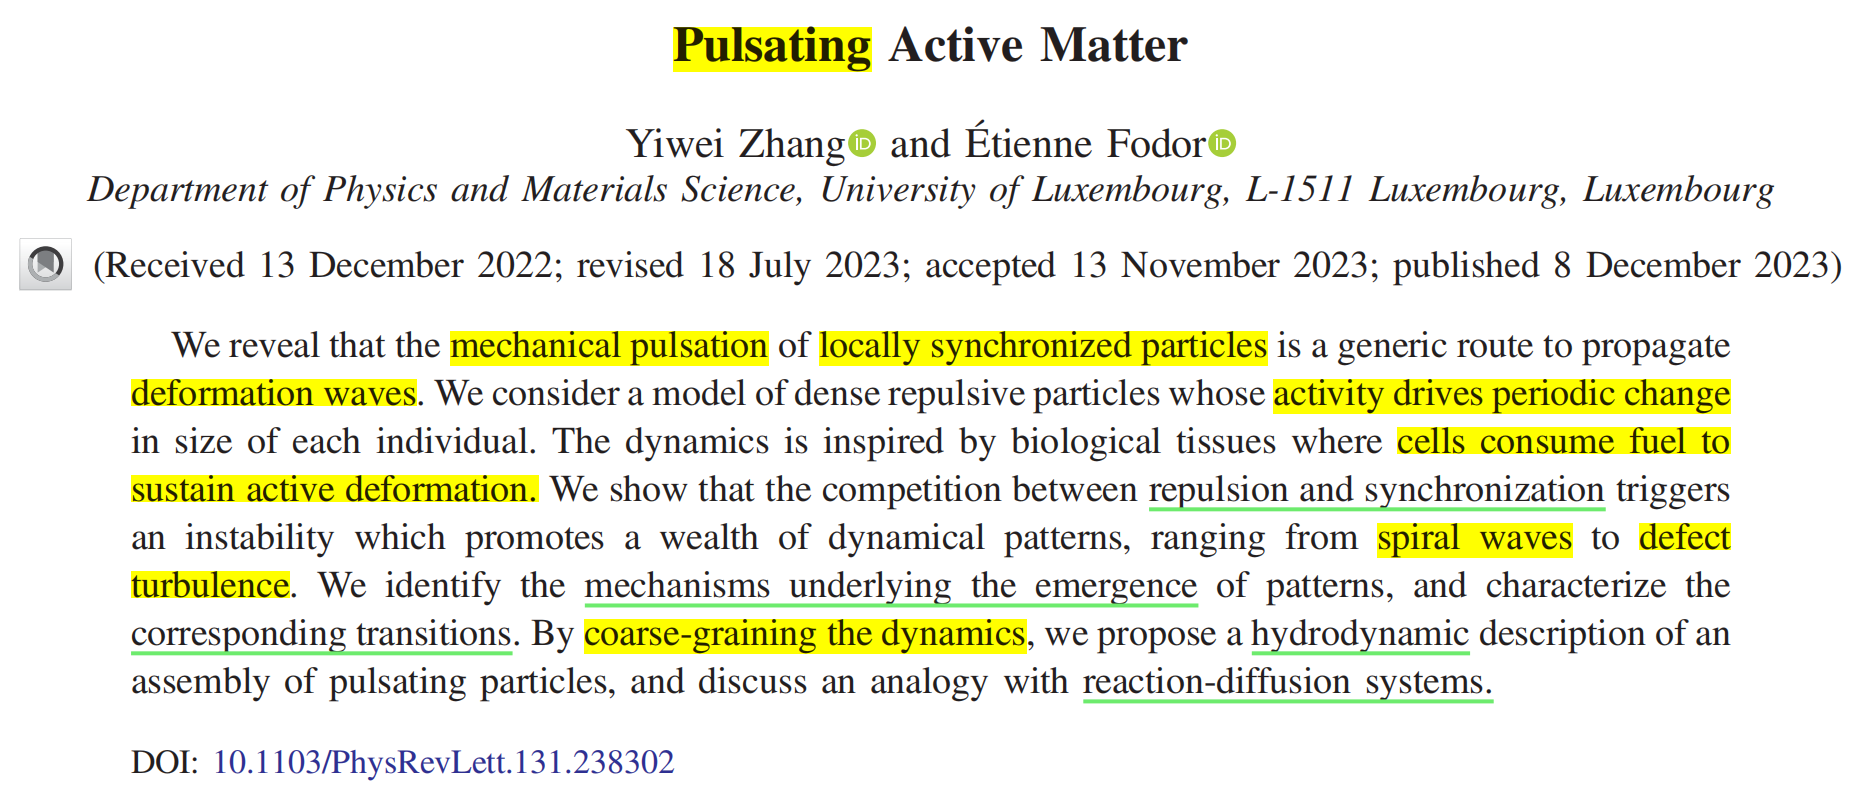
\includegraphics[width=\textwidth]{figs/title2.png}
\end{frame}

\begin{frame}
    \begin{multicols}{2}
    
        {\scriptsize
        $$
        \begin{aligned}
            \dot{\mathbf{r}}_i&=-\mu \sum_j{\partial _{\mathbf{r}_i}U\left( a_{ij} \right) +\sqrt{2D}\xi _i}\\
            \dot{\theta}_i&=\omega -\sum_j{\left[ \tau \left( a_{ij},\theta _i-\theta _j \right) +\mu _{\theta}\partial _{\theta _i}U\left( a_{ij} \right) \right] +\sqrt{2D_{\theta}}\eta _i}\\
        \end{aligned}
        $$
        }

        {
        \scriptsize
    
        $$
        \begin{aligned}
            a_{ij}&=\frac{\left| \mathbf{r}_i-\mathbf{r}_j \right|}{\sigma \left( \theta _i \right) +\sigma \left( \theta _j \right)}\\
            \sigma \left( \theta _i \right) &=\sigma _0\frac{1+\lambda \sin \theta _i}{1+\lambda}\\
            U\left( a \right) &=\begin{cases}
            U_0\left( a^{-12}-2a^{-6} \right) ,&		a<1\\
            0,&		\mathrm{otherwise}\\
        \end{cases}\\
            \tau \left( a,\theta \right) &=\begin{cases}
            \varepsilon \sin \left( \theta \right) ,&		a<1\\
            0,&		\mathrm{otherwise}\\
        \end{cases}\\
        \end{aligned}
        $$

        $$
        \begin{aligned}
            \varphi &=\pi \sum_{i=1}^N{\left[ \sigma \left( \theta _i \right) /L \right] ^2}\\
            r&=\frac{1}{N}\left| \sum_{j=1}^N{e^{\mathrm{i}\theta _j}} \right|\\
        \end{aligned}
        $$

        \begin{tabular}{ll}
            Symbols& Meanings \\
            \hline
            $\mathrm{r}$ & position \\
            $\theta$ & phase, \\
             & determining the particle size \\
            $U$ & pairwise repulsive potential \\
            $\mu$ & self-propulsion mobility \\
            $D$ & diffusivity \\
            $\xi$ & isotropic Gaussian white noise \\
            $\sigma(\theta)$ & particle size \\
            $\sigma_0$ & largest size \\
            $\lambda<1$ & pulsation amplitude \\
        \end{tabular}
        }

    \end{multicols}

\end{frame}

\begin{frame}
    \begin{multicols}{2}
        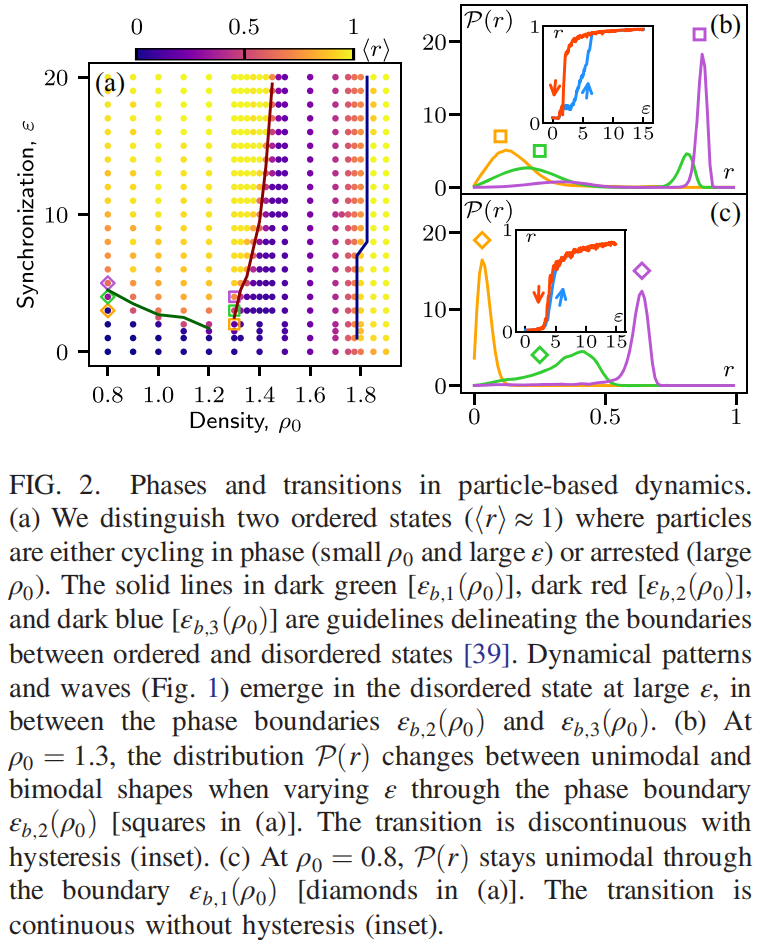
\includegraphics[width=0.5\textwidth]{figs/p2_f2.png}

        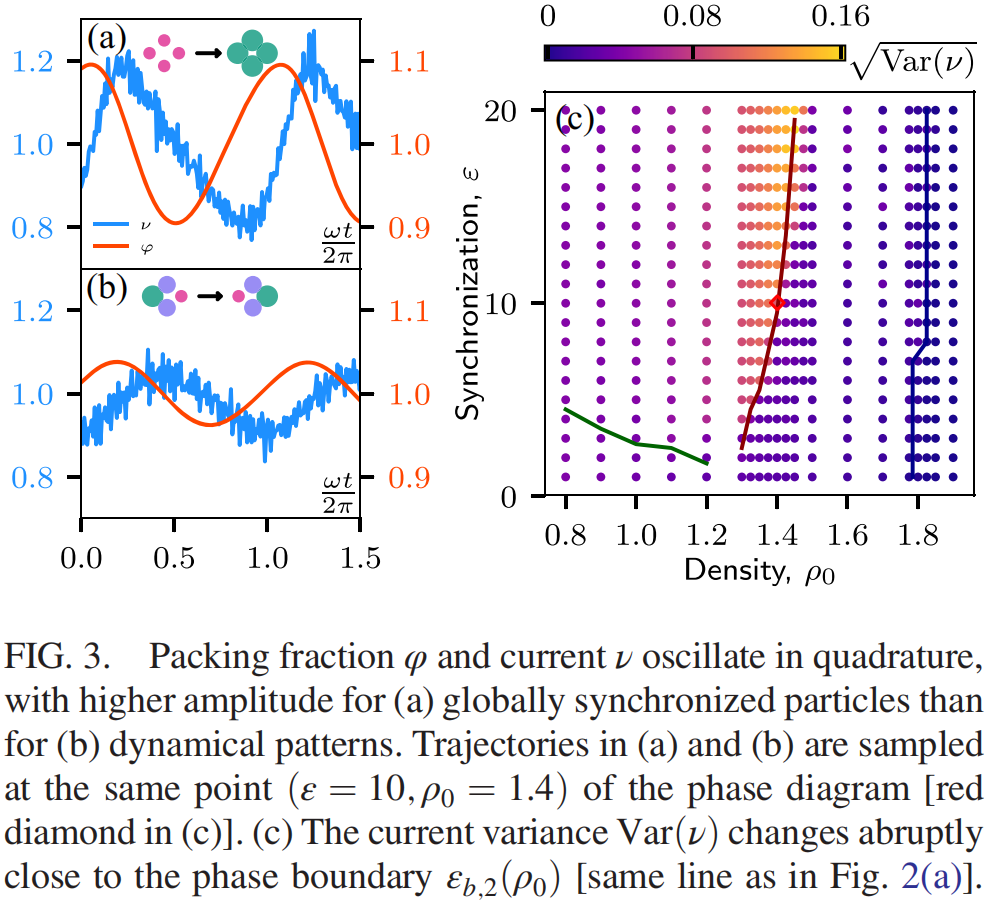
\includegraphics[width=0.5\textwidth]{figs/p2_f3.png}
    \end{multicols}
\end{frame}

\begin{frame}
    \begin{multicols}{2}
        {
        \tiny
            $$
            \begin{aligned}
                \partial _tA&=\left( \frac{\bar{\varepsilon}\rho _0}{2}-D_{\theta}+\mathrm{i}\omega +D\nabla ^2 \right) A-\frac{\bar{\varepsilon}^2A\left| A \right|^2}{4\left( 2D\theta -\mathrm{i}\omega \right)}\\
                &-\mathrm{i}cA\left[ \mathrm{Re}\left( A \right) +\frac{\bar{\varepsilon}\lambda}{4}\mathrm{Im}\left( \frac{A^2}{2D\theta -\mathrm{i}\omega} \right) \right] +\sqrt{\rho _0D_{\theta}}\Lambda\\
            \end{aligned}
            $$
        }
        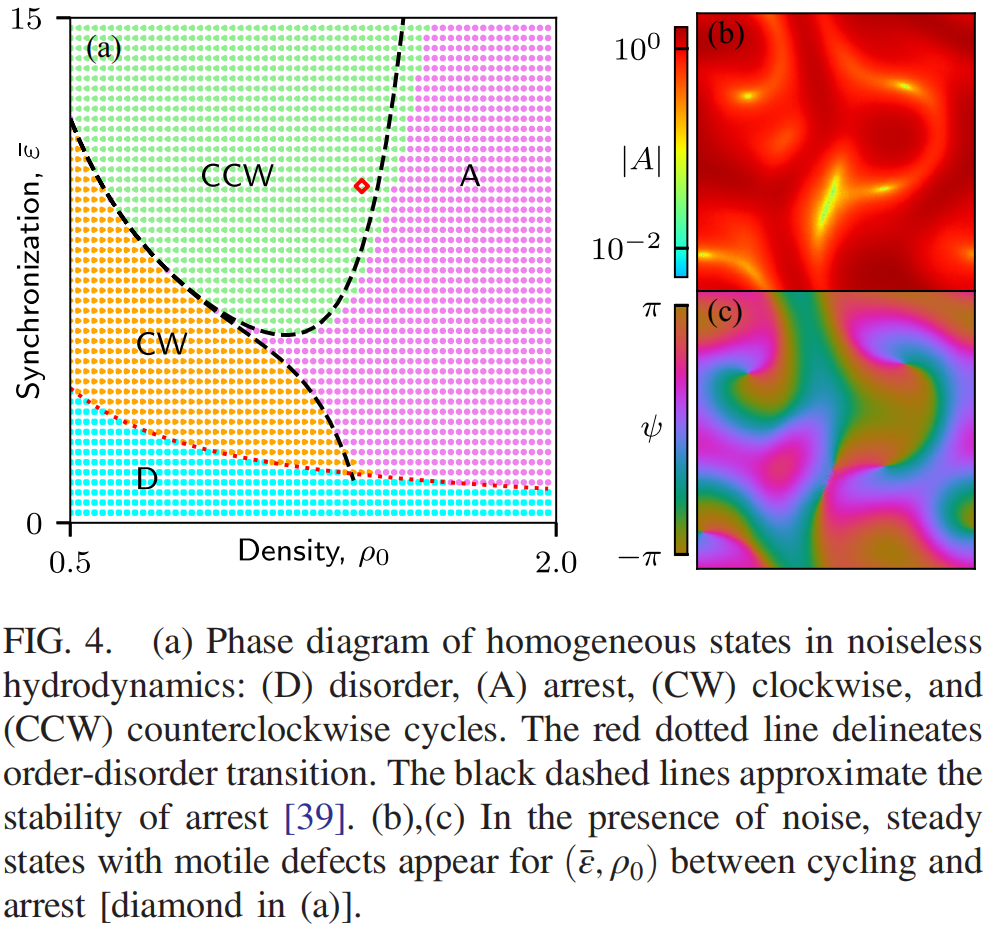
\includegraphics[width=0.5\textwidth]{figs/p2_f4.png}
    \end{multicols}
\end{frame}

% -----------------------------------------------------------------------------
\end{document}

